\chapter{Introduction}\label{sec-introduction}
Before there were mobile devices, there was media content. But now that there are mobile devices, 
there is even more media content, and both media content consumption and generation lie at the heart of mobile applications. 

For thousands of years, people have never exhausted their desire to feast their eyes on something visually and ``illusionally'' attractive (see Figure~\ref{fig:visual-feasts}). 
Since photography and television devices were invented, people have begun to spend more and more time on virtual scenes in front of their eyes, be it a photograph, a movie screen, a TV screen, a PC monitor, a tablet PC, a smartphone, or a VR\footnote{Virtual Reality. Example phenomenal device: Oculus of Facebook.} headset.  
Small wonder that VR and AR\footnote{Augmented Reality. Example killer app: Pokemon Go by Niantic.} are subsequently and concurrently two of the hottest topics in consumer electronics today. 
\begin{figure}[ht]
	\centering
	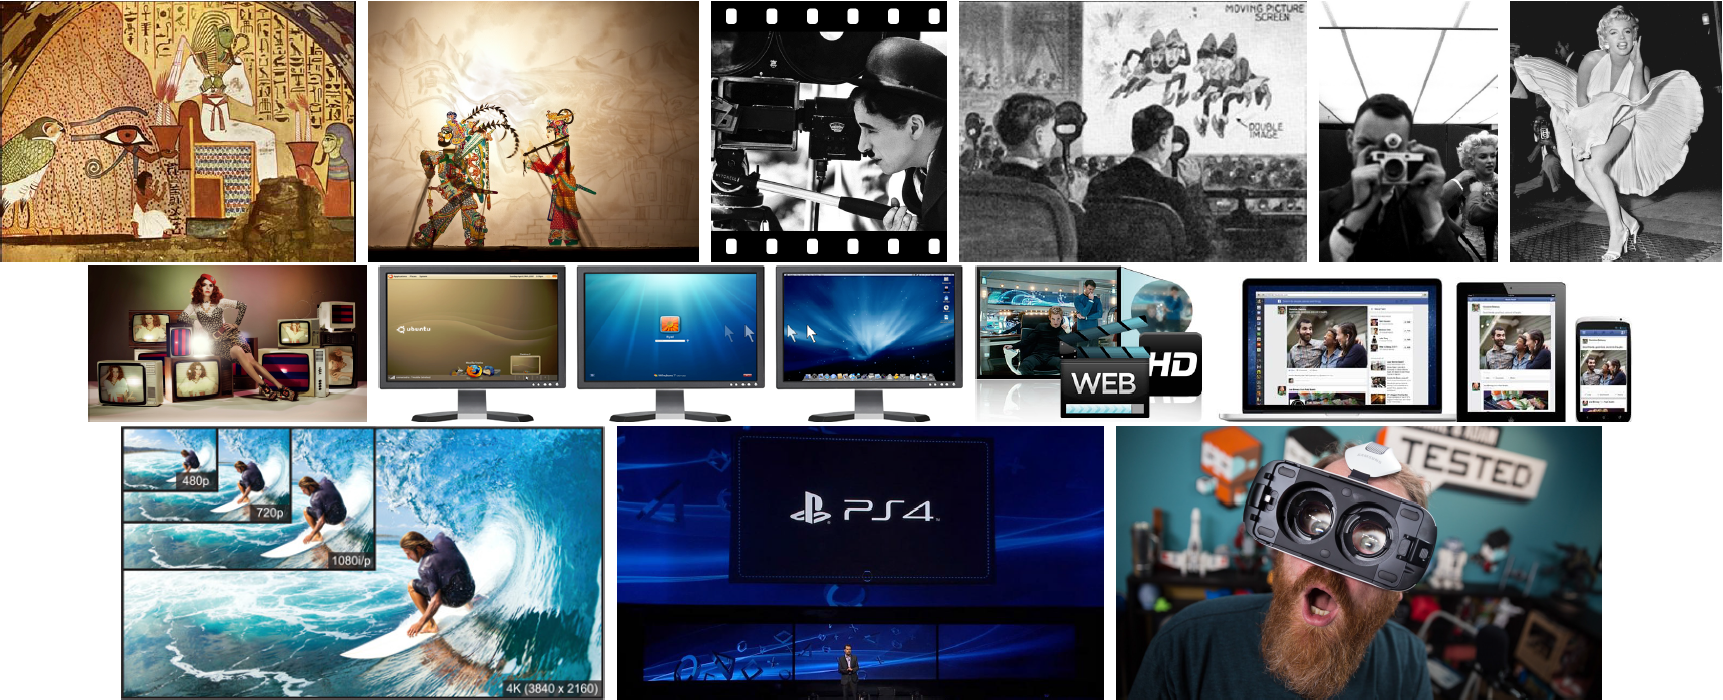
\includegraphics[width=\linewidth]{fig/general/visual-feasts.png}
	\caption{Human's visual feasts in history.}\label{fig:visual-feasts}
\end{figure}

Billions of people now enjoy huge screens and high definition videos. For entertainment,  people are now greedily expecting to experience as many details in the virtual world as in reality. 
This is why nowadays we have 720p, 1080p, 2K, and 4K resolution pictures and videos, with 8K to 16K coming in the near future. 
Moreover, since VR technology tends to be prevalent in gaming and entertainment, billions of mobile devices are ready to fetch these super high definition VR videos from the Internet to please their masters. 
For Internet television, the elementary-level resolution is 1080p and the standard-level is 4K; in VR/AR, 4K is considered basic, while it is expected that the standard-level will soon become 16K. 

What kind of network throughput problems will we face with the rise and rapid use of VR/AR devices? Figure~\ref{fig:bitrate-resolution} roughly illustrates the relationship between the resolutions and the bitrates required with the H.265 (HEVC) coding standard. 

\begin{figure}[ht]
	\centering
	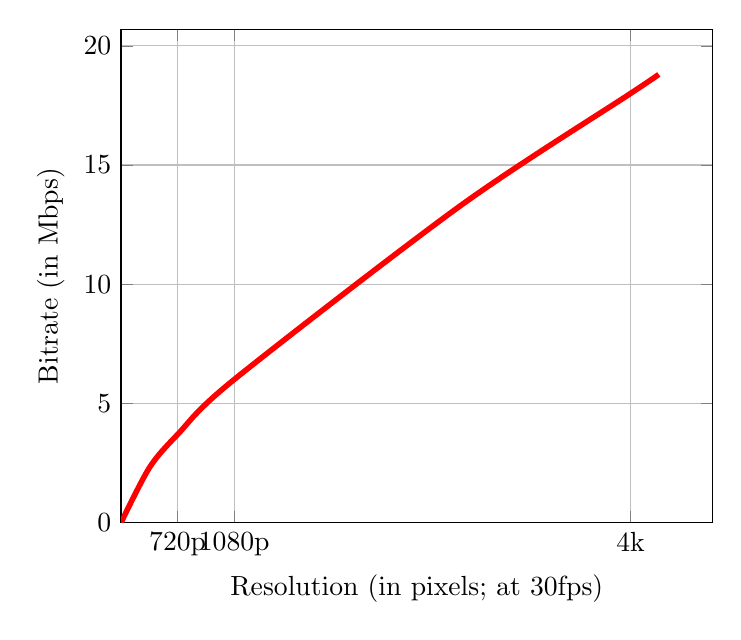
\begin{tikzpicture} %[>=latex]
\begin{axis}[
width=0.75\textwidth,
%line width=2,
%symbolic x coords={2012, 2013, 2014, 2015, 2016},
xtick={2,4,18},
xticklabels={720p,1080p,4k},
%minor xtick={0,1,...,18},
grid=both,
ymin=0,
xmin=0,
xlabel=Resolution (in pixels; at 30fps),
ylabel=Bitrate (in Mbps),
%enlarge x limits=0.1,
%xticklabel style={text width=0.2\textwidth,align=flush left},
]
\addplot[line width=2pt,smooth,color=red] coordinates {
	(0,0)
	(1,2.300)
	(2,3.700)
	%(3,5050)
	(4,6.006)
	(12,13.300)
	(18,18.000)
	(19,18.800)
};
%\draw[red] plot [smooth] coordinates {(0 0) (2,3700) (4,6006) (18,18000)};
\end{axis}
\end{tikzpicture}
	\caption{Bandwidth required for delivering various videos.}\label{fig:bitrate-resolution}
\end{figure}

To put this in perspective, let's look at the coming explosion in demand for network throughput. With the rapid progress of low-power wireless communications and the evolution of micro-sensors, the not-really-new concept of IoT begins to touch ground in novel fields like smart wearables, smart agriculture, smart homes, smart buildings, smart environments, smart cities, smart transportation, smart enterprises and smart hospitality. It is an undoubted trend that there will be an exponentially growing number of devices connecting to the Internet. 
In 2011, Cisco predicted that there would be 25 billion devices connected to the Internet by 2015 and 50 billion by 2020 \cite{evans2011internet}. 

Just imagine if these devices continually send 1K total-sized \texttt{HeartBeat} messages to the cloud in 1-second intervals. 
What kind of pressure will this put on backbone networks and cloud services in general? What challenges will network engineers face in coming years? And what new solutions will emerge? 

These challenges have forced the emergence of fog computing, a fairly new paradigm which basically moves some elements of Cloud Computing closer to the end users, especially in a machine-to-machine (M2M), collaborative platform; these elements include compute, storage, and networking devices \cite{Bonomi:2012:Fog:IoT}. 

Pear Limited, hereinafter referred to as ``Pear'', is an innovative start-up company that originated at the \emph{Foggy University}\footnote{It is a homophone of HKUST in Cantonese, because people in Hong Kong call it ``Foh Gei Dai Hok''; ``Foh Gei'' sounds like ``Foggy'' and means ``Science and Technology'', while ``Dai Hok'' means ``University''. Interestingly, every spring the HKUST campus is rather foggy because of its proximity to the sea. This fact makes the university live up to its ``Foggy'' nickname.} campus and mainly focuses on implementing fog computing technology from concept to reality. The business idea leverages future technological trends to meet real needs. 

Research on fog computing is still in its very early stages. On 19 November 2015, ARM, Cisco, Dell, Intel, Microsoft and Princeton University formed the OpenFog Consortium. It plans to set up seven different working groups aiming at solving problems in fog computing, but so far it has only published one architectural white paper\footnote{\url{https://github.com/OpenFog/white-papers/tree/master/Architecture}}. Therefore, Pear is neither required nor able to address all aspects of fog computing. Pear will first follow, implement, and practise a specific category of fog --- a relatively ``stable'' kind of fog, serving in-between the Clouds and the clients. It hopes it can get a foothold in this new market before the rules are established and before too many giant players join the game.

From one angle, Pear Fog is a descending cloud --- a pool of compute, networking and storage resources across the core through to the edge of the Internet. From another point of view, Pear Fog is a new and improved powerful peer-to-peer (P2P) system incorporated within a crowd-sourced paradigm, providing Infrastructure as a Service (IaaS), Platform as a Service (PaaS), or Software as a Service (SaaS) in a ``Uber''-like way. 
In addition, Pear Fog is compatible with and complementary to existing clouds. One of its goals is to serve as a coordinator of Cloud-Fog coordinators. 

We plan to implement and operate a business-friendly subset of fog with crowdsourcing that will help some giant CPs and CDNs cut their costs and provide better services to end-users. Hereinto, the end-users can pair with Pear to form a pool of computational resources. 
Pear will schedule the resources to process business tasks and rebate a portion of its profits to the end-users accordingly. 

To provide stable and sufficient fog services, Pear has to source and distribute a large number of fog devices powered by Pear's software, and it has several strategies to do so. %as well as to choose what and how to do carefully. 

This thesis documents the following three contributions:
\begin{itemize}
	\item It presents a thorough survey of related fields along the pathway from the early days of networking to the Cloud to the Fog. 
	\item It proposes several effective approaches to offer fog services, in terms of software framework, network design, use cases, {\em etc.}
	\item It describes approaches to scale up the fog network, actualise the technologies, and from some mutually beneficial alliances to get off the ground and survive as a viable business in a cutthroat market. 
\end{itemize} 

We present an in-depth historical analysis of related areas. From the rises and falls of different technologies, as well as the ups and downs of different concepts, we share illuminating lessons. From these lessons, we summarise the key points and identify the best practices.   
The lessons stated in Chapter~\ref{sec-his-analysis} have inspired our decisions. 

We have decided to implement a business-friendly subset of fog first. We then provide further details on what we have chosen to do. Using analogy reasoning, we have arrived at a resolution to initially focus on single critical endeavour: implementing a multi-functional WebRTC gateway in C language. To make this business feasible, we need a stable hardware carrier with sufficient storage. We further analyse the types of fog resources and their dominant battlefields, and we generalise all the crowdsourcing fog services' model. We also analyse where fog will serve better than cloud, especially for content delivery. Finally we conclude by three medium-term projects. Thus, Chapter~\ref{sec-decisions} comes why, what and how we will develop our software and hardware products. 

To create a sustainable business, we carefully consider various product, price, place, promotion, partnership, and funding and financial plans. These are presented in Chapter~\ref{chp-biz-analysis}. 
